\scanpage{35}

(1.8) Considérons enfin les pts fixes

\[
\deleted{\beta_0}\inserted{\alpha'(0)}=2,\qquad
\deleted{\beta_1}\inserted{\alpha'(1)}=-1,\qquad
\deleted{\beta_\infty}\inserted{\alpha'(\infty)}=\tfrac12
\tag*{(32)}
\]

\figure{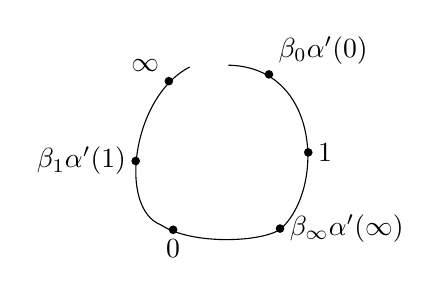
\begin{tikzpicture}[scale=.78]
\draw (0.62,2.75) .. controls (-.32,2.27) and (-.55,.45) .. (.15,.18) .. controls (.67,-.16) and (1.83,-.10) .. (2.11,.12) .. controls (2.82,.78) and (2.74,2.75) .. (1.25,2.78);
\fill (.28,2.52) circle(2pt) node[above left] {$\infty$};
\fill (1.91,2.63) circle(2pt) node[above right] {$\deleted{\beta_0}\alpha'(0)$};
\fill (2.55,1.36) circle(2pt) node[right] {$1$};
\fill (2.09,.12) circle(2pt) node[right] {$\deleted{\beta_\infty}\alpha'(\infty)$};
\fill (.35,.10) circle(2pt) node[below] {$0$};
\fill (-.26,1.22) circle(2pt) node[left] {$\deleted{\beta_1}\alpha'(1)$};
\end{tikzpicture}}

qui sont les pts fixes, autres que $0,1,\infty$ resp., des transpositions $\tau_0,\tau_1,\tau_\infty\in\unsure{\mathfrak S_3|\mathscr S_3}$. Soit

\[
\boxed{\deleted{\unsure{\beta'_*}}\alpha'_*=\{\deleted{\beta_0}\alpha'(0),\deleted{\beta_1}\alpha'(1),\deleted{\beta_2}\alpha'(2)\}.}
\tag*{(33)}
\]

On veut déterminer $E(\deleted{\beta'_*}\alpha'_*)\inserted{=\coprod_{i\in I}E(\deleted{\beta_i}\alpha'(i))}$ comme $\mathcal E$-ensemble.

On trouve

\[
\left\{\begin{aligned}
E_n(\deleted{\beta_i}\alpha'(i))&\simeq\{(\unsure{\zeta|\xi}_j)\in\overline{\mathbb Q}^{I\setminus\{i\}}\mid \zeta_j^n=-\tfrac12\quad\forall j\in I\setminus\{i\}\}\\
&\simeq K_n(-\tfrac12)^{I\setminus\{i\}}\\
E(\deleted{\beta_i}\alpha'(i))&\simeq K(-\tfrac12)^{I\setminus\{i\}}
\end{aligned}\right.\tag*{(34)}
\]

où $\forall\,\unsure{\zeta_0|\xi_0|g}\in\overline{\mathbb Q}$, on pose

\[
\left\{\begin{aligned}
K_n(\zeta)&=\{\zeta\in\overline{\mathbb Q}\mid\zeta^n=\zeta_0\}\\
K_\infty(\zeta)&=K(\zeta)=\varprojlim_n K_n(\zeta)
\end{aligned}\right.\tag*{(35)}
\]

$K_\infty(\zeta)$ étant un torseur sous $T=\mu_\infty$, sur lequel $\Gamma$ opère (donc un $\deleted{\unsure{(T,|\mathrm{Ext}}}(\mu_\infty,\Gamma)$-torseur ...)

Ici on aura, en vertu des \unsure{rel. can.|iso. can.}

\[
K(\zeta\unsure{\zeta'|g'} )\deleted{\unsure{\circ}}\simeq K(\zeta)\wedge_{\unsure{\Pi_\infty|T}}K(\zeta')
\]

\[
K(-\tfrac12)\simeq K(-1)\wedge_T K(\tfrac12)\simeq K(-1)\wedge_T K(2)^{-1}
\tag*{(36)}
\]

\[
\underset{\wr\,p_2^{-1}(\{-1\})}{K(-1)}\lhook\joinrel\longrightarrow\deleted{\unsure{E_0}}T,\qquad
(1\mathrel{-}T\mathrel{\overset{2}{-}}T\mathrel{\overset{p_2}{-}}\mu_2\longrightarrow\unsure{1|0})
\tag*{(37)}
\]

% archive sheet number: 34
